\documentclass[11pt]{article}
\usepackage[utf8]{inputenc}
\usepackage[T1]{fontenc}
\usepackage{amsmath, bm}
\usepackage{float}
\usepackage{hyperref, tikz}
\usepackage{bm}
\usepackage{tikz}
\usepackage{caption}
\usepackage{subcaption}
\usepackage{mathtools}
\usepackage{verbatim}

\usetikzlibrary{calc}
\setcounter{secnumdepth}{0}
\DeclareMathOperator{\relu}{ReLU}
\DeclareMathOperator{\sign}{sign}
\begin{document}
\begin{center}
  \mbox{}\\[2.0cm]
  \textsc{\Huge Deep Learning}\\[1.0cm]
  \textsc{\Large Homework 1}\\[0.5cm]
\end{center}
\begin{flushleft}
  Group 71 members: \\[0.5cm]
  \begin{itemize}
  \item Luis Jose De Macedo Guevara (95621)
  \item Vincent Jakl (108529)
  \end{itemize}
\end{flushleft}

\section{Contributions of each member}
\begin{itemize}
    \item Luis Jose De Macedo Guevara (95621):
    \item Vincent Jakl (108529):
\end{itemize}
\pagebreak
\section{Question 1}
\subsection{1. a)}
The single perceptron was not the best choice for this task.
As can be seen in Figure \ref{fig:single_layer_perceptron} below, the perceptron was not able to fit to the high dimensional data also with no sign of improvement.
With the 20 epochs, it ended up with a 0.3422 test accuracy which is slightly higher than 0.25 that would happen with random selection for 4 classes.
Also the learning rate was left at the value of 1 so this might cause the problem as well.
\begin{figure}[h!]
  \centering
  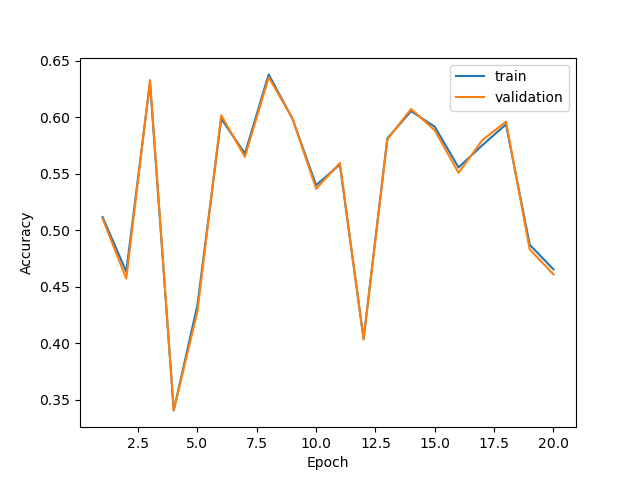
\includegraphics[width=0.75\textwidth]{./plots/single_perceptron.png}
  \caption{Single perceptron}\label{fig:single_layer_perceptron}
\end{figure}

\subsection{1. b)}
The logistic regression performed better than the single perceptron.
As can be seen in Figure \ref{fig:logistic_regression}, the logistic regression was able to fit to the data better.
There was however a big difference between the two learning rates.
Where the model with the learning rate of 0.01 jumped faster to the higher accuracy, it did not improve on a regular basis.
The 0.001 lr model was a bit slower to get up to higher accuracy, but it was able to consistently improve.
In the end the 0.01 lr model ended up with 0.5784 test accuracy and the 0.001 lr model ended up with 0.5936 test accuracy.
Running these models for more epochs would possibly improve the accuracy since the training was still showing signs of improvement even with the evaluation metric.

\begin{figure}[h!]
\centering
\begin{subfigure}{.5\textwidth}
  \centering
  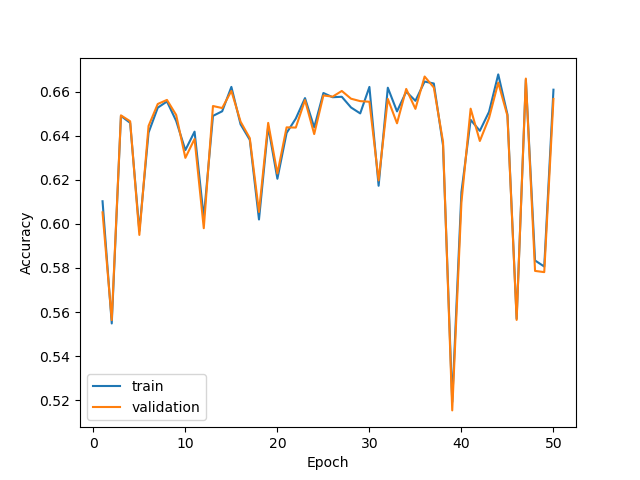
\includegraphics[width=\linewidth]{./plots/logistic_regression_0.01.png}
  \caption{lr 0.01}
  \label{fig:sub1}
\end{subfigure}%
\begin{subfigure}{.5\textwidth}
  \centering
  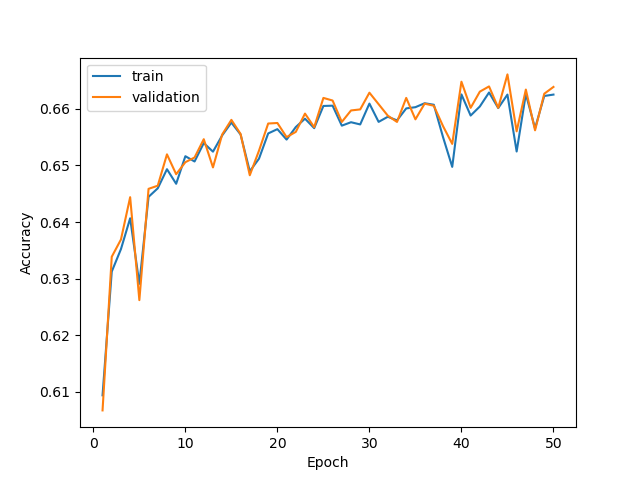
\includegraphics[width=\linewidth]{./plots/logistic_regression_0.001.png}
  \caption{lr 0.001}
  \label{fig:sub2}
\end{subfigure}
\caption{Logistic regression}
\label{fig:logistic_regression}
\end{figure}

\subsection{2. a)}
We do believe that the statement is correct.
The multilayer perceptron can be more expressive than logistic regression.
The logistic regression is a linear model and therefore it can only learn linear decision boundaries.
The multilayer perceptron can learn non-linear decision boundaries due to the $\relu$ activation.
However, the logistic regression is a convex optimization problem whereas an MLP generally is not, making it easier to train and find the global minima in logistic regression.

\subsection{2. b)}
As seen Figure \ref{fig:mlp2b}, we can see that the multilayer perceptron, as specified, is a better fit for the data, not only its accuracy on both training and validation data largely improves with each epoch, so does its training loss. It also shows a good test accuracy of $0.7580$ after $20$ epochs. Looking at the trend in both graphs, we can expect a better accuracy on the training/validation data with more epochs and possibly, taking care to avoid overfitting, a better testing accuracy.
\begin{figure}[h!]
\centering
\begin{subfigure}{.5\textwidth}
  \centering
  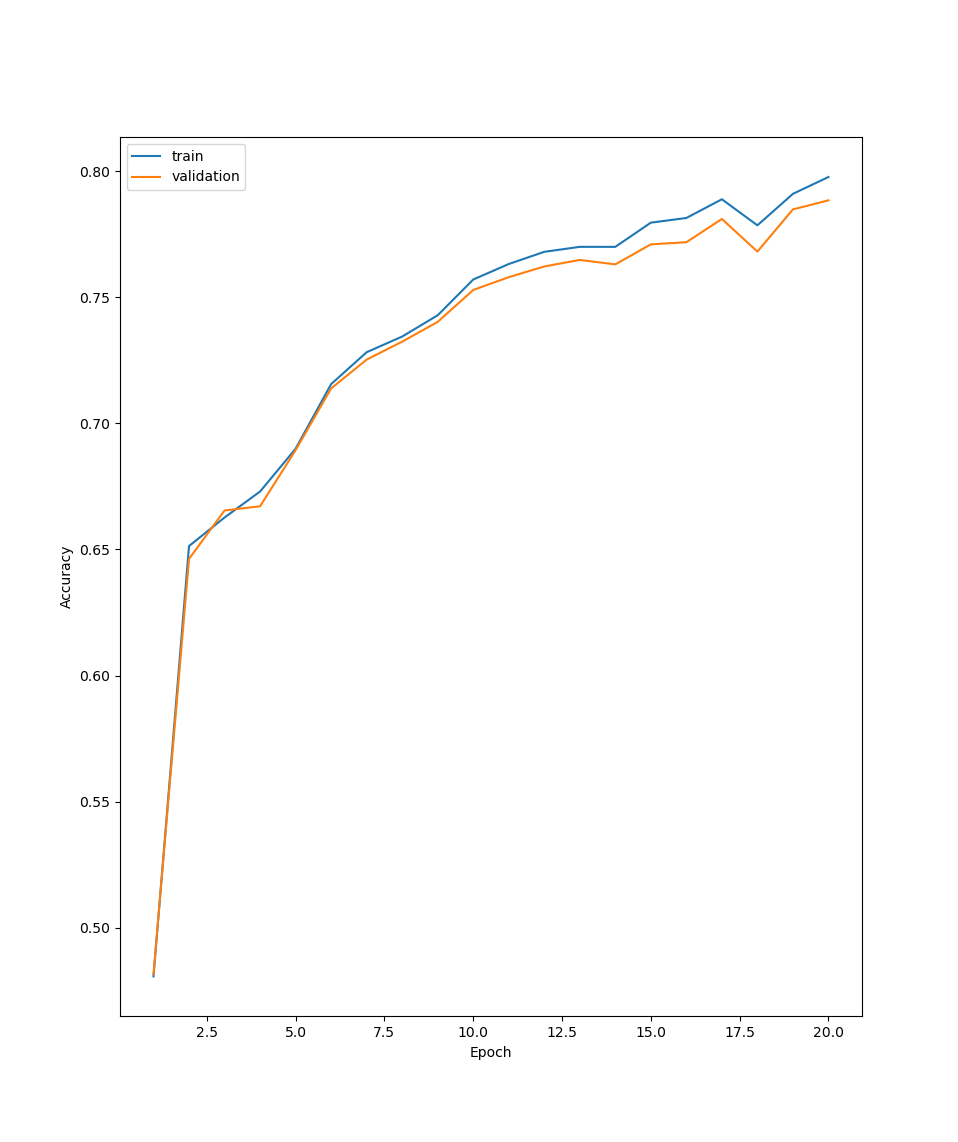
\includegraphics[width=.9\linewidth]{./plots/mlp_acc_per_epoch.png}
  \caption{Training/Validation accuracy per epoch}
\end{subfigure}%
\begin{subfigure}{.5\textwidth}
  \centering
  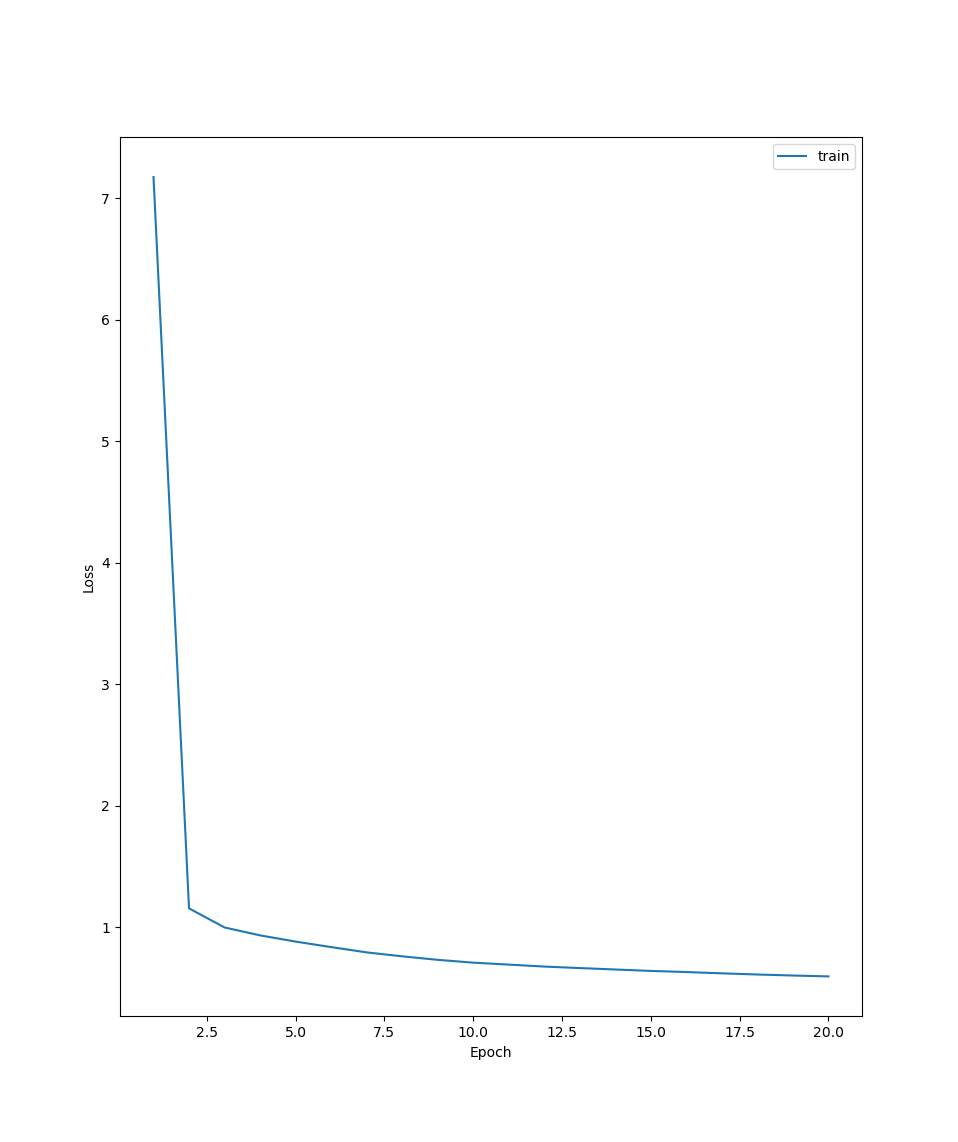
\includegraphics[width=.9\linewidth]{./plots/mlp_loss_per_epoch.png}
  \caption{Loss as a function of epoch number}
\end{subfigure}
\caption{MLP w/o Pytorch}
\label{fig:mlp2b}
\end{figure}

\clearpage

\section{Question 2}
\subsection{1.}
After implementing the logistic regression with Pytorch, the best performing learning rate was 0.001 with the final test accuracy of 0.6503.
All the test accuracies are as follows 0.5577, 0.6200, 0.6503 in the order of learning rate 0.1, 0.01, 0.001.
Again here it looks like 20 training epochs were not enough to get the best performance out of the model.
%In the graphs below, it is visible that the model was still improving on the training data.
%Also it is noticable, how the 0.1 learning rate model had maybe too high of a learning rate since on the graph, the validation accuracy is jumping all around.
\begin{comment}
  \begin{figure}[h!]
    \centering
    \begin{subfigure}{.5\textwidth}
      \centering
      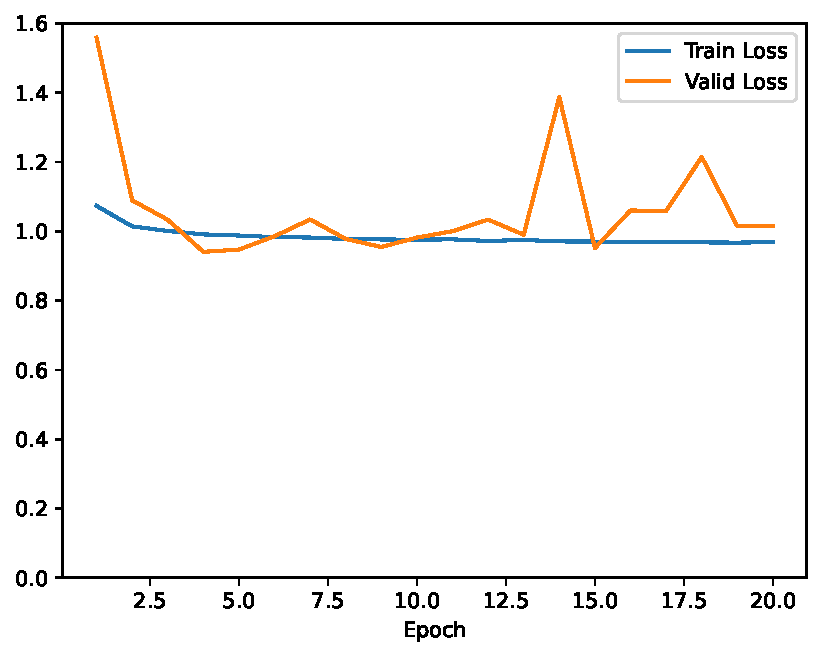
\includegraphics[width=.9\linewidth]{plots/logistic_regression-training-loss-batch-16-lr-0.1-epochs-20-l2-0-opt-sgd}
      \caption{Training/Validation loss per epoch}
    \end{subfigure}%
    \begin{subfigure}{.5\textwidth}
      \centering
      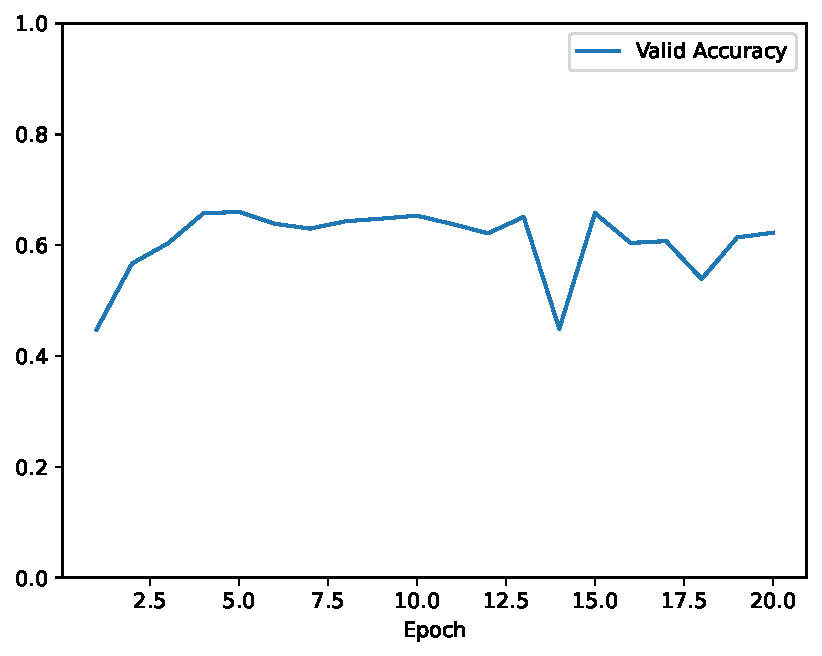
\includegraphics[width=.9\linewidth]{plots/logistic_regression-validation-accuracy-batch-16-lr-0.1-epochs-20-l2-0-opt-sgd}
      \caption{Validation accuracy per epoch}
    \end{subfigure}
    \caption{Logistic regression lr 0.1}
    \label{fig:regression_lr_0.1}
  \end{figure}

  \begin{figure}
    \centering
    \begin{subfigure}{.5\textwidth}
      \centering
      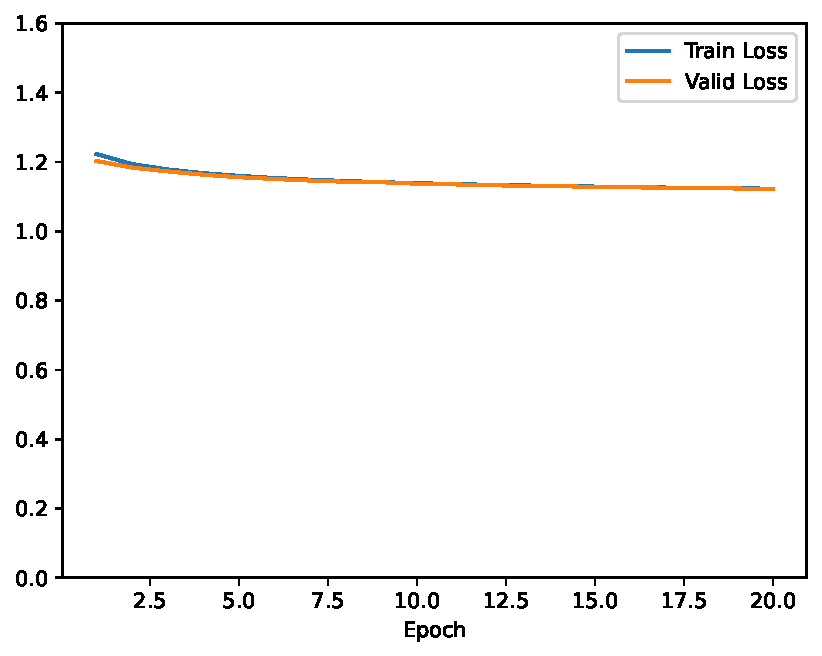
\includegraphics[width=.9\linewidth]{plots/logistic_regression-training-loss-batch-16-lr-0.01-epochs-20-l2-0-opt-sgd}
      \caption{Training/Validation loss per epoch}
    \end{subfigure}%
    \begin{subfigure}{.5\textwidth}
      \centering
      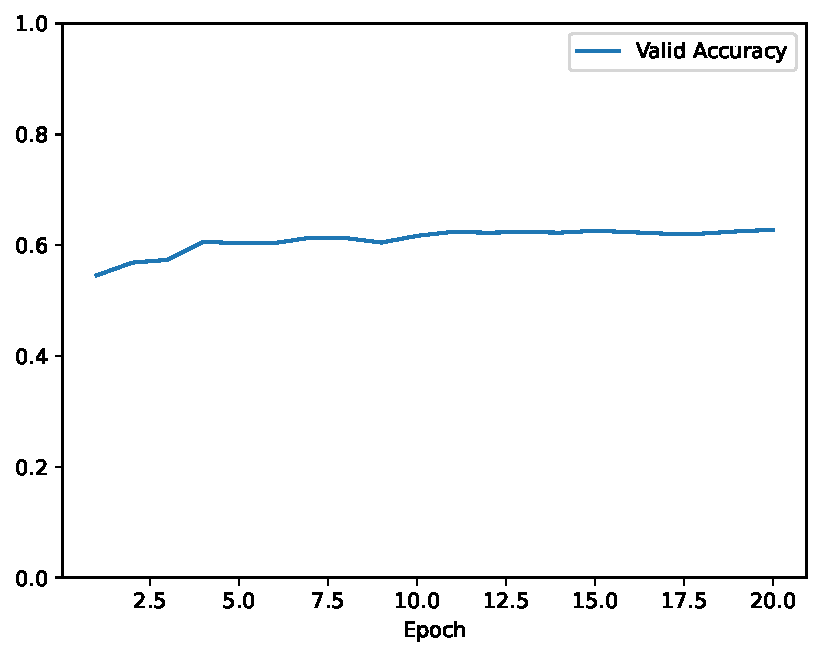
\includegraphics[width=.9\linewidth]{plots/logistic_regression-validation-accuracy-batch-16-lr-0.01-epochs-20-l2-0-opt-sgd}
      \caption{Validation accuracy per epoch}
    \end{subfigure}
    \caption{Logistic regression lr 0.01}
    \label{fig:regression_lr_0.01}
  \end{figure}
\end{comment}
\begin{figure}[h!]
\centering
\begin{subfigure}{.5\textwidth}
  \centering
  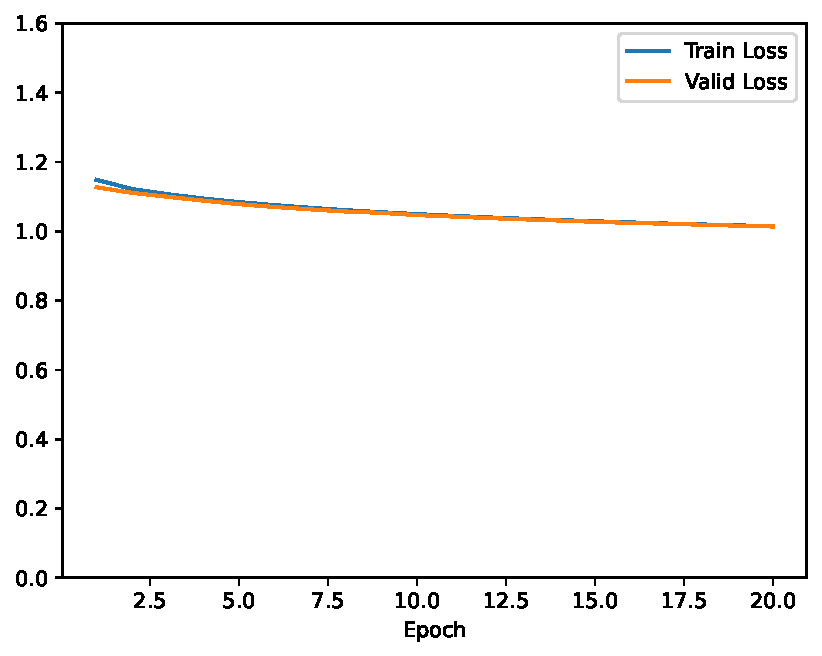
\includegraphics[width=.9\linewidth]{plots/logistic_regression-training-loss-batch-16-lr-0.001-epochs-20-l2-0-opt-sgd}
  \caption{Training/Validation loss per epoch}
\end{subfigure}%
\begin{subfigure}{.5\textwidth}
  \centering
  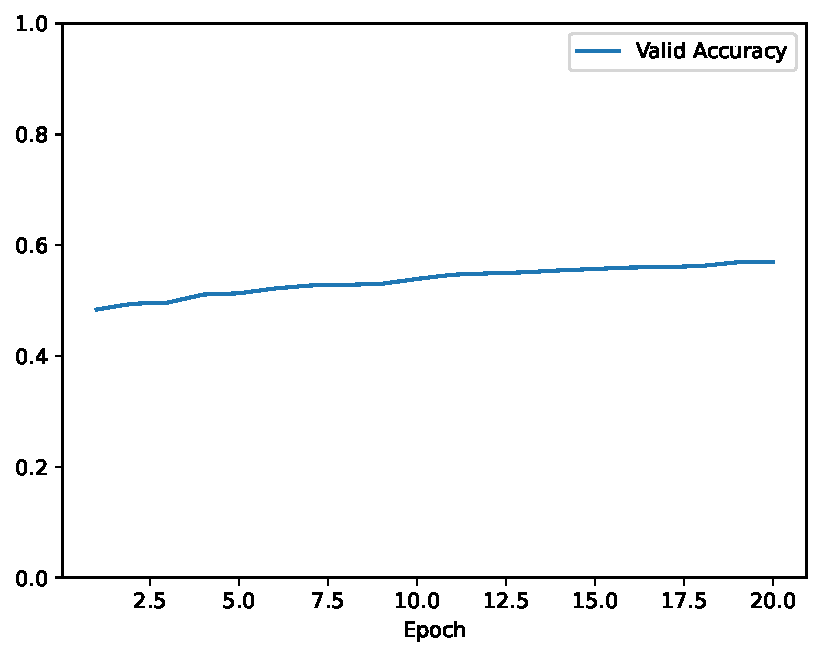
\includegraphics[width=.9\linewidth]{plots/logistic_regression-validation-accuracy-batch-16-lr-0.001-epochs-20-l2-0-opt-sgd}
  \caption{Validation accuracy per epoch}
\end{subfigure}
\caption{Logistic regression lr 0.001}
\label{fig:regression_lr_0.001}
\end{figure}

\pagebreak

\subsection{2. a)}
When training the MLP with Pytorch, the batch size of 16 trained slower than the batch size of 1024.
The 16 batch size finished in $678$ seconds whereas the 1024 batch size finished in $353$ seconds.
However, since the 16 batch size trained on overally more batches, it was able to perform a little bit better
The final testing accuracy of the 16 batch size was $0.7372$ whereas the 1024 batch size was $0.7183$.
Once again we can see here, that more epochs would probably improve the performance of the model.

\begin{figure}[h!]
\centering
\begin{subfigure}{.5\textwidth}
  \centering
  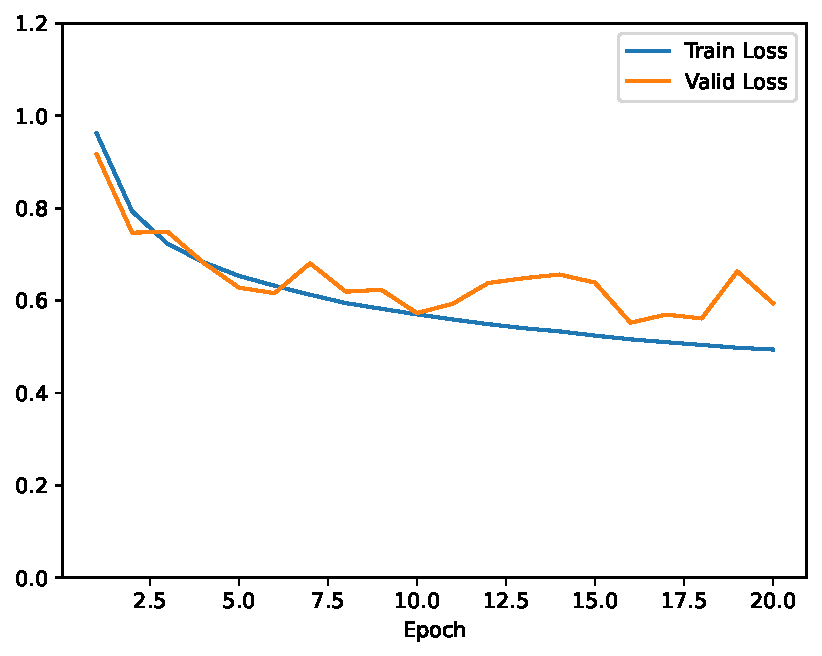
\includegraphics[width=.9\linewidth]{plots/mlp-training-loss-batch-16-lr-0.1-epochs-20-hidden-200-dropout-0-l2-0-layers-1-act-relu-opt-sgd}
  \caption{Training/Validation loss per epoch}
\end{subfigure}%
\begin{subfigure}{.5\textwidth}
  \centering
  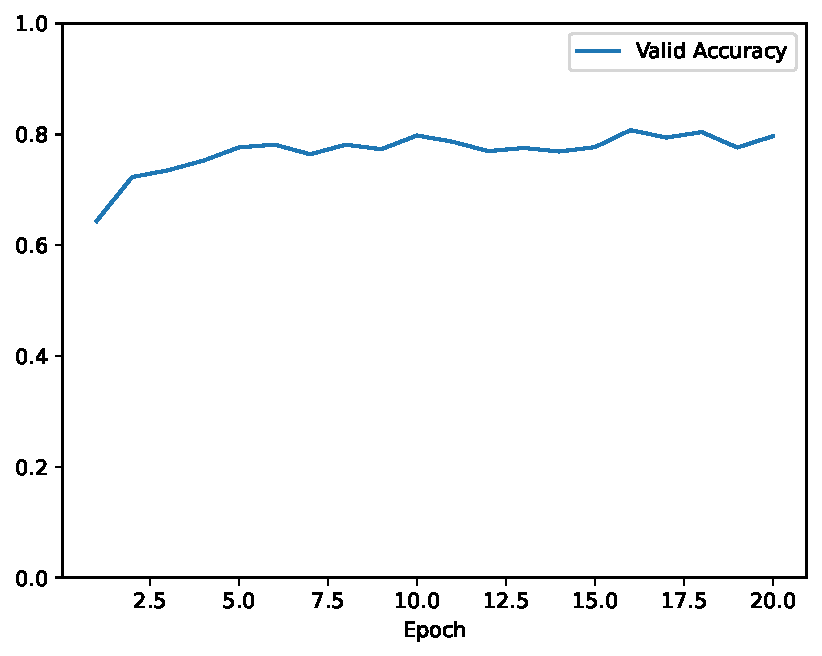
\includegraphics[width=.9\linewidth]{plots/mlp-validation-accuracy-batch-16-lr-0.1-epochs-20-hidden-200-dropout-0-l2-0-layers-1-act-relu-opt-sgd}
  \caption{Validation accuracy per epoch}
\end{subfigure}
\caption{MLP batch size 16}
\label{fig:MLP_batch_size_16}
\end{figure}

\begin{figure}[h!]
\centering
\begin{subfigure}{.5\textwidth}
  \centering
  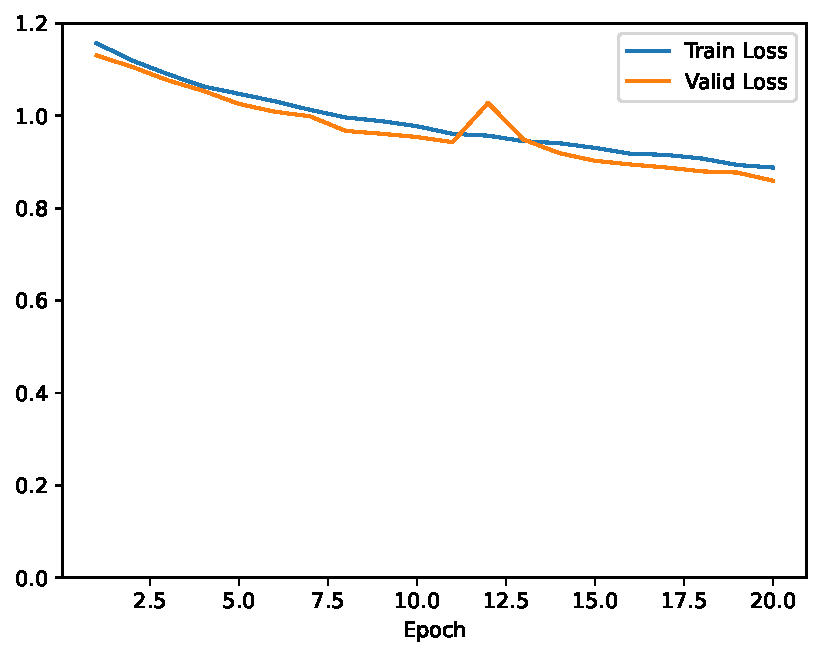
\includegraphics[width=.9\linewidth]{plots/mlp-training-loss-batch-1024-lr-0.1-epochs-20-hidden-200-dropout-0-l2-0-layers-1-act-relu-opt-sgd}
  \caption{Training/Validation loss per epoch}
\end{subfigure}%
\begin{subfigure}{.5\textwidth}
  \centering
  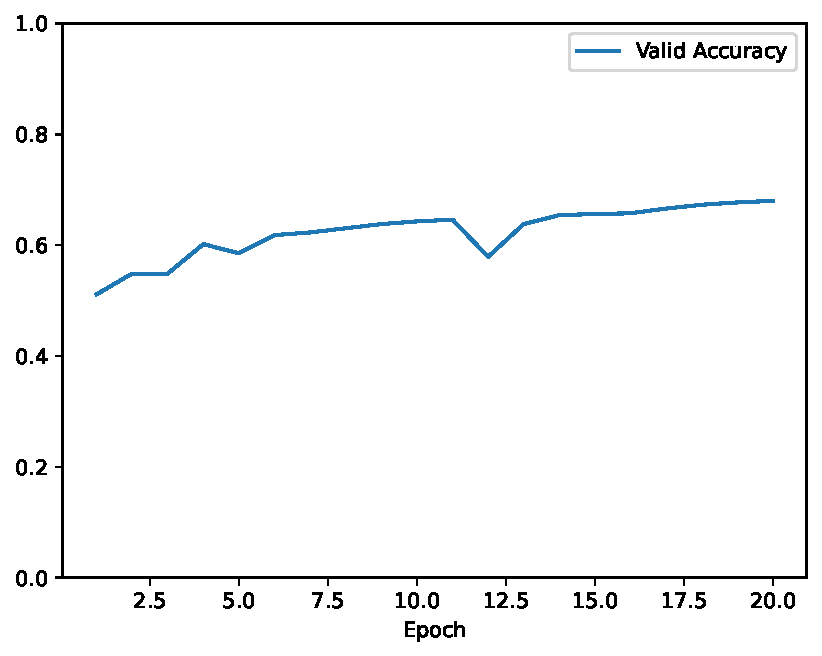
\includegraphics[width=.9\linewidth]{plots/mlp-validation-accuracy-batch-1024-lr-0.1-epochs-20-hidden-200-dropout-0-l2-0-layers-1-act-relu-opt-sgd}
  \caption{Validation accuracy per epoch}
\end{subfigure}
\caption{MLP batch size 1024}
\label{fig:MLP_batch_size_1024}
\end{figure}

\subsection{2. b)}
Out of the four learning rates, the worst performing one was lr 1. This makes sense, since the gradient descent probably overshoots the minimum.
The best performing learning rate was 0.01 with the final test accuracy of $0.7580$, whereas the learning rate of 1 had the final test accuracy of $0.4726$.

\begin{figure}[h!]
\centering
\begin{subfigure}{.5\textwidth}
  \centering
  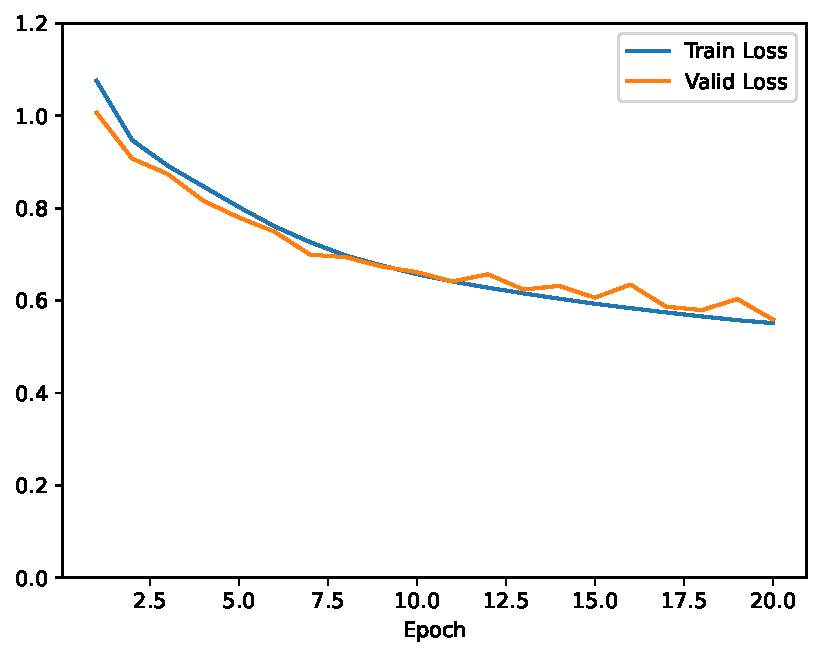
\includegraphics[width=.9\linewidth]{plots/mlp-training-loss-batch-16-lr-0.01-epochs-20-hidden-200-dropout-0-l2-0-layers-1-act-relu-opt-sgd}
  \caption{Training/Validation loss per epoch}
\end{subfigure}%
\begin{subfigure}{.5\textwidth}
  \centering
  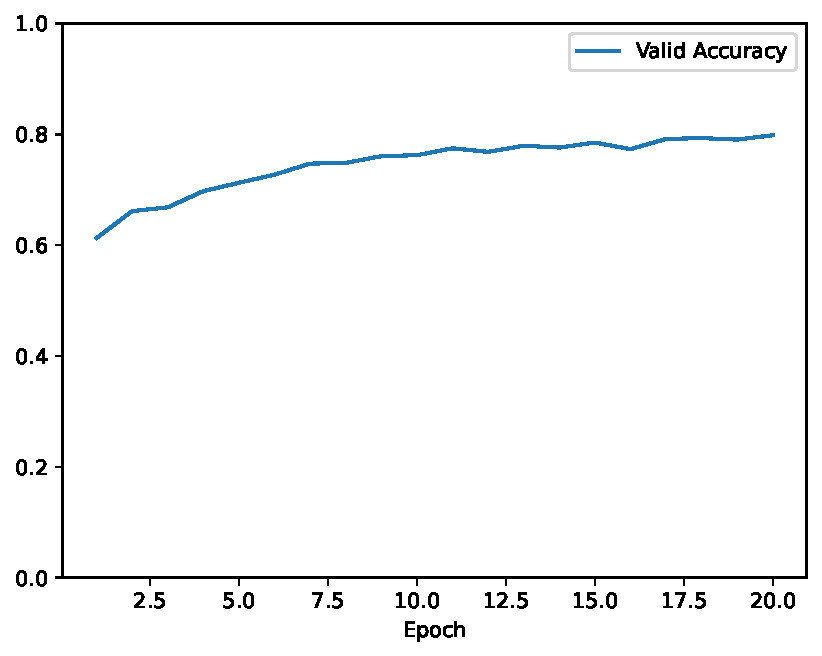
\includegraphics[width=.9\linewidth]{plots/mlp-validation-accuracy-batch-16-lr-0.01-epochs-20-hidden-200-dropout-0-l2-0-layers-1-act-relu-opt-sgd}
  \caption{Validation accuracy per epoch}
\end{subfigure}
\caption{MLP lr 0.01}
\label{fig:MLP_lr_0.01}
\end{figure}

\begin{figure}[h!]
\centering
\begin{subfigure}{.5\textwidth}
  \centering
  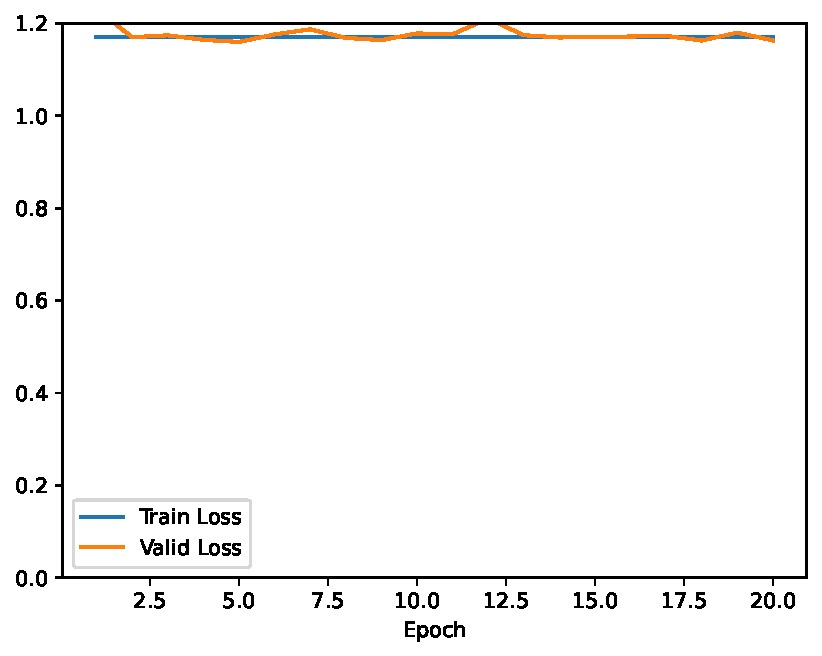
\includegraphics[width=.9\linewidth]{plots/mlp-training-loss-batch-16-lr-1.0-epochs-20-hidden-200-dropout-0-l2-0-layers-1-act-relu-opt-sgd}
  \caption{Training/Validation loss per epoch}
\end{subfigure}%
\begin{subfigure}{.5\textwidth}
  \centering
  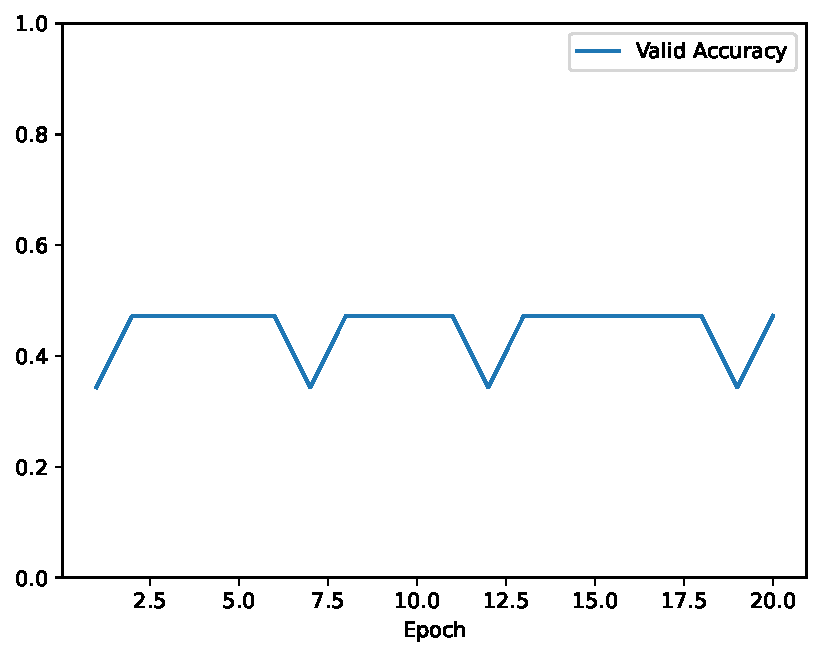
\includegraphics[width=.9\linewidth]{plots/mlp-validation-accuracy-batch-16-lr-1.0-epochs-20-hidden-200-dropout-0-l2-0-layers-1-act-relu-opt-sgd}
  \caption{Validation accuracy per epoch}
\end{subfigure}
\caption{MLP lr 1}
\label{fig:MLP_lr_1}
\end{figure}

\subsection{2. c)}
When training the network for 150 epochs and 256 batch size, the model gets to higher accuracies than the previous models.
However in the training/validation loss graph (Figure \ref{fig:MLP_overfitting}) we can see, that the training and validation loss start to diverge after around 60 epochs.
This is a sign of overfitting.
When comparing the L2 regularization and dropout regularization, the better final test accuracy is the one with the L2 regularization.
However the dropout regularization train/validation loss graph looks like it would still benefit from more training, since the training and validation loss are both still improving, and not diverging.
The final test accuracy for the L2 regularization was $0.7864$ and for the dropout regularization it was $0.7845$.
This makes both the models, the best performing models out of all the models trained in this question.
\begin{figure}[h!]
\centering
\begin{subfigure}{.5\textwidth}
  \centering
  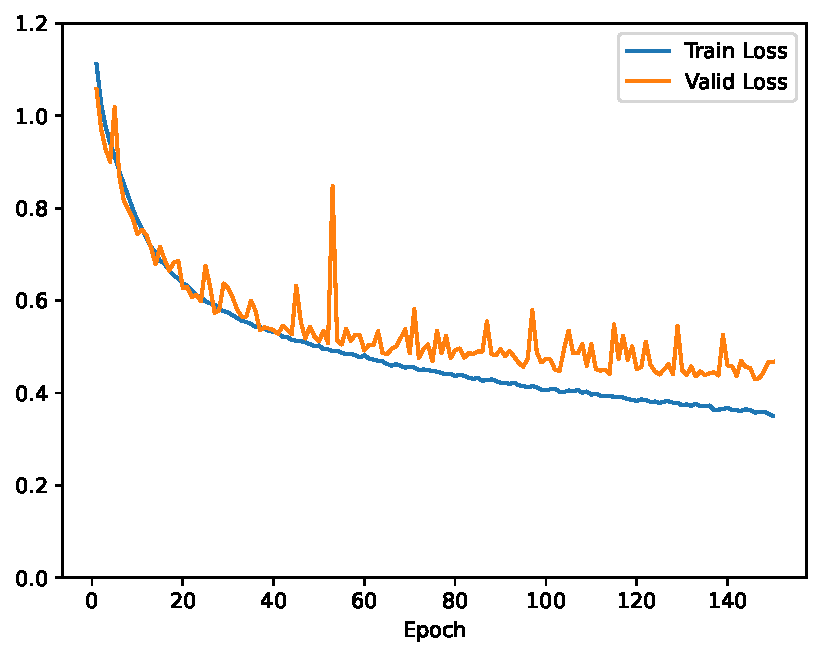
\includegraphics[width=.9\linewidth]{plots/mlp-training-loss-batch-256-lr-0.1-epochs-150-hidden-200-dropout-0-l2-0-layers-1-act-relu-opt-sgd.pdf}
  \caption{Training/Validation loss per epoch}
\end{subfigure}%
\begin{subfigure}{.5\textwidth}
  \centering
  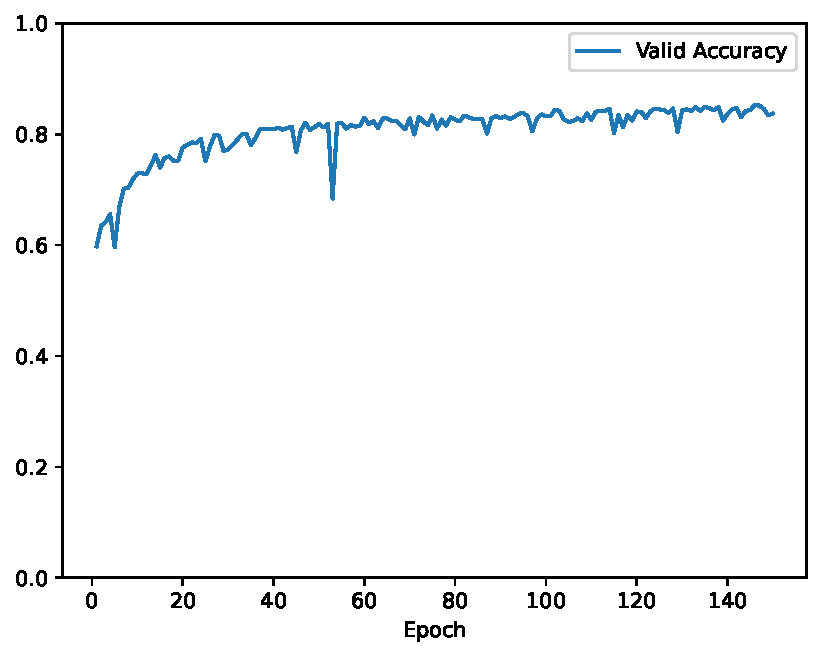
\includegraphics[width=.9\linewidth]{plots/mlp-validation-accuracy-batch-256-lr-0.1-epochs-150-hidden-200-dropout-0-l2-0-layers-1-act-relu-opt-sgd}
  \caption{Validation accuracy per epoch}
\end{subfigure}
\caption{MLP overfitting}
\label{fig:MLP_overfitting}
\end{figure}
\begin{figure}[h!]
\centering
\begin{subfigure}{.5\textwidth}
  \centering
  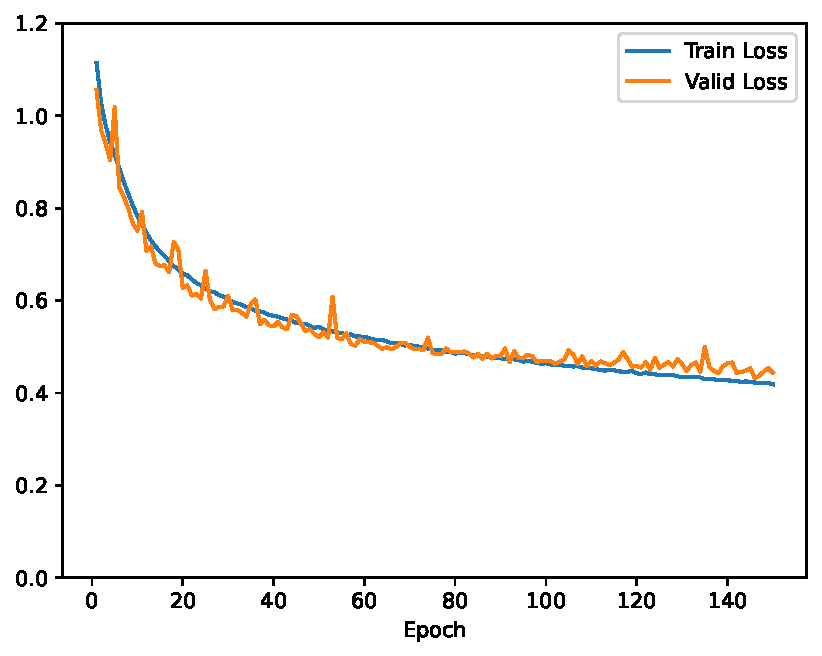
\includegraphics[width=.9\linewidth]{plots/mlp-training-loss-batch-256-lr-0.1-epochs-150-hidden-200-dropout-0.2-l2-0-layers-1-act-relu-opt-sgd.pdf}
  \caption{Training/Validation loss per epoch}
\end{subfigure}%
\begin{subfigure}{.5\textwidth}
  \centering
  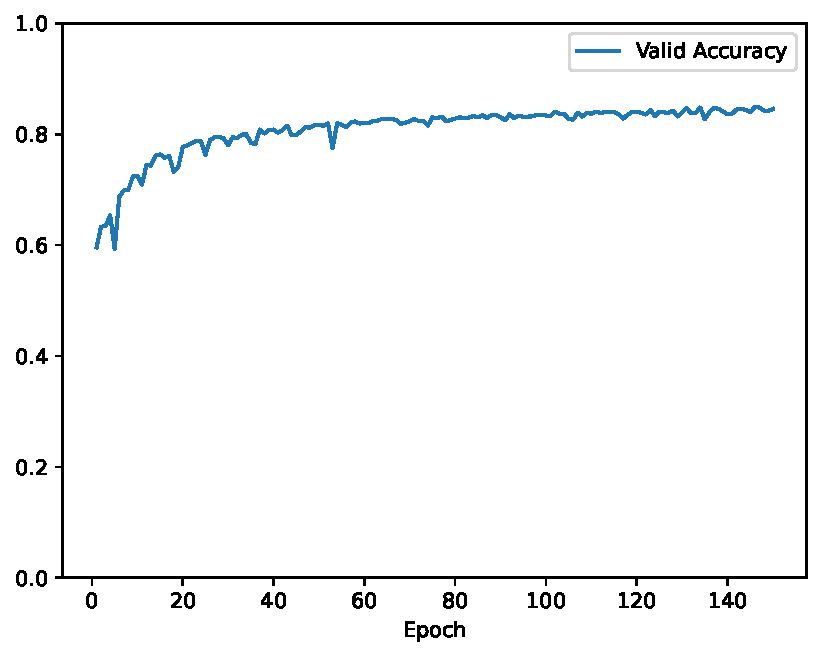
\includegraphics[width=.9\linewidth]{plots/mlp-validation-accuracy-batch-256-lr-0.1-epochs-150-hidden-200-dropout-0.2-l2-0-layers-1-act-relu-opt-sgd}
  \caption{Validation accuracy per epoch}
\end{subfigure}
\caption{MLP dropout}
\label{fig:MLP_dropout}
\end{figure}

\begin{figure}[h!]
\centering
\begin{subfigure}{.5\textwidth}
  \centering
  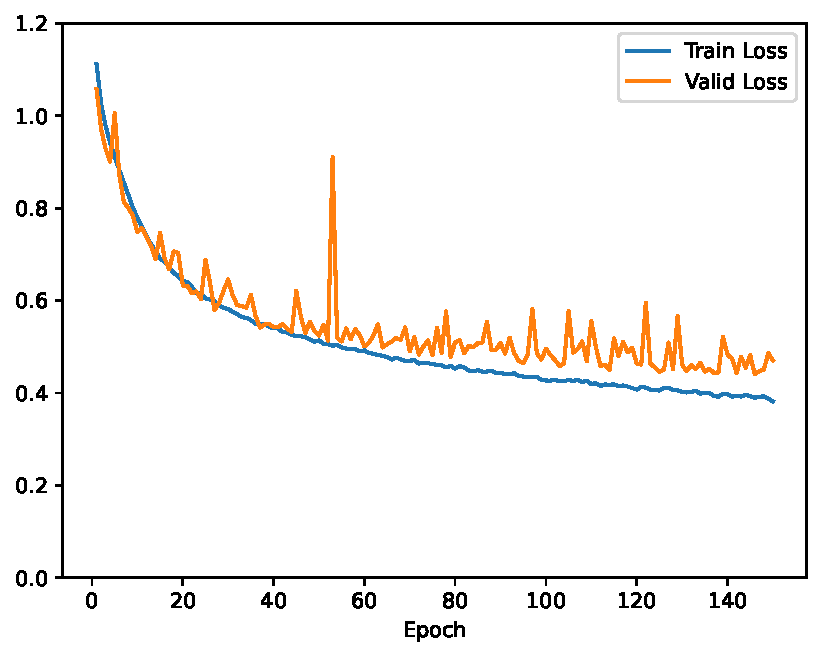
\includegraphics[width=.9\linewidth]{plots/mlp-training-loss-batch-256-lr-0.1-epochs-150-hidden-200-dropout-0-l2-0.0001-layers-1-act-relu-opt-sgd.pdf}
  \caption{Training/Validation loss per epoch}
\end{subfigure}%
\begin{subfigure}{.5\textwidth}
  \centering
  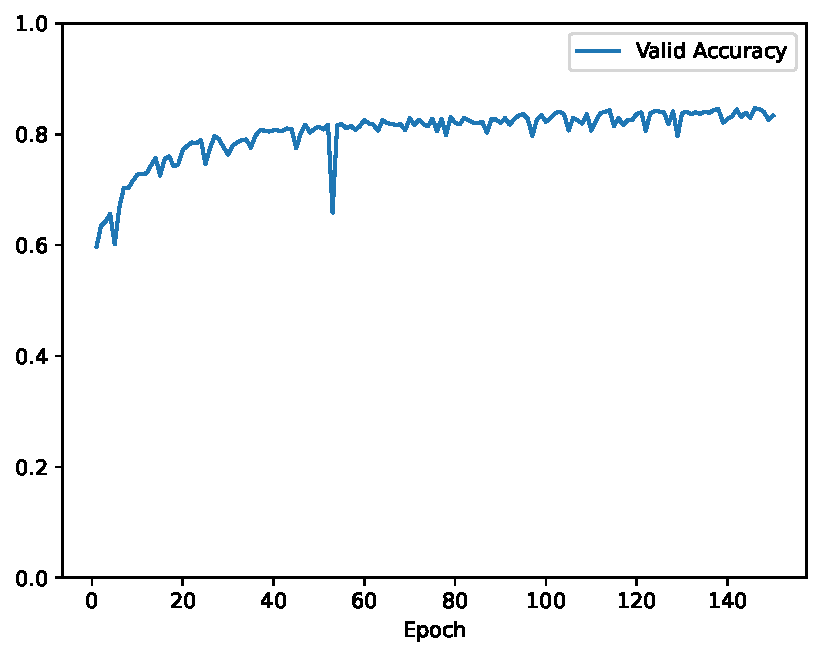
\includegraphics[width=.9\linewidth]{plots/mlp-validation-accuracy-batch-256-lr-0.1-epochs-150-hidden-200-dropout-0-l2-0.0001-layers-1-act-relu-opt-sgd}
  \caption{Validation accuracy per epoch}
\end{subfigure}
\caption{MLP L2 regularization}
\label{fig:MLP_L2_regularization}
\end{figure}

\clearpage

\section{Question 3}
\subsection{1.}
\subsubsection{a)}
Let
\begin{itemize}
  \item $D = 2$
  \item $A = B = 0$
  \item $\bm{x}^{(1)} = \begin{bmatrix} 1 \\ 1\end{bmatrix}$, $\bm{x}^{(2)} = \begin{bmatrix} 1 \\ -1\end{bmatrix}$, $\bm{x}^{(3)} = \begin{bmatrix} -1 \\ 1\end{bmatrix}$ and $\bm{x}^{(4)} = \begin{bmatrix} -1 \\ -1\end{bmatrix}$, 
  \end{itemize}
  We have $f ( \bm{x}^{(1)}) = -1$, $f ( \bm{x}^{(2)}) = +1$, $f ( \bm{x}^{(3)}) = +1$ and $f ( \bm{x}^{(4)}) = -1$

  \begin{figure}[H]
  \begin{tikzpicture}[xscale=2, yscale=2, domain=0.140:60,samples=800]
    \draw[->] (-2, 0) -- (2, 0) node[right] {$x$};
    \draw[->] (0, -2) -- (0, 2) node[above] {$y$};
    \foreach \i in {-1, 1} {
        \draw (\i, 0.05) -- (\i, -0.05) node[below] {$\i$};
        \draw (0.05, \i) -- (-0.05, \i) node[left] {$\i$};
    }

    \node[red, scale=1.5] at (1, 1) {\textbullet};
    \node[green, scale=1.5] at (-1, 1) {\textbullet};
    \node[green, scale=1.5] at (1, -1) {\textbullet};
    \node[red, scale=1.5] at (-1, -1) {\textbullet};
  \end{tikzpicture}
  \end{figure}
  Which we can see is not linearly separable and therefore a perceptron cannot learn a separating hyperplane.

\pagebreak

\subsubsection{b)}
\begin{figure*}[h!]
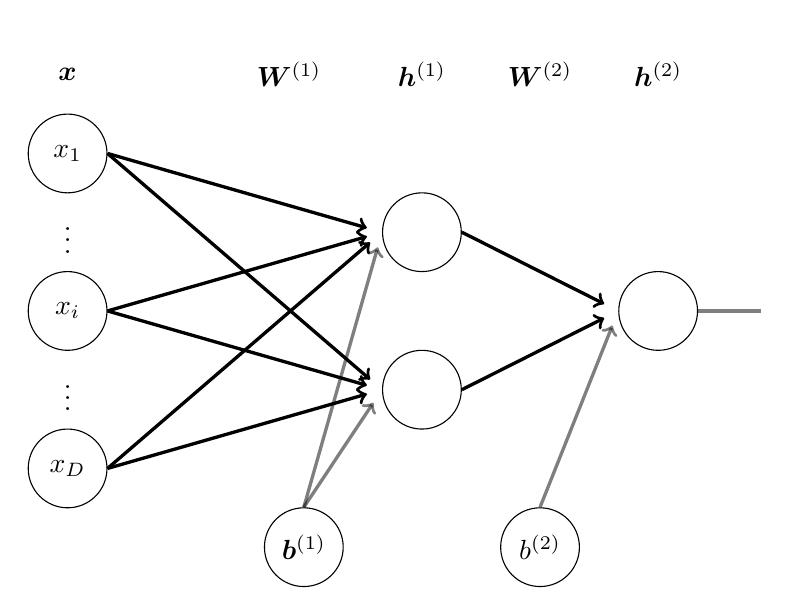
\begin{tikzpicture}
  \draw (0, 0) node[circle, minimum size=10mm, draw] (x1) {$x_{1}$};
  \draw ($(x1) - (0, 1)$) node[circle, minimum size=10mm] (xd1) {$\vdots$};
  \draw ($(xd1) - (0, 1)$) node[circle, minimum size=10mm, draw] (xi) {$x_{i}$};
  \draw ($(xi) - (0, 1)$) node[circle, minimum size=10mm] (xd2) {$\vdots$};
  \draw ($(xd2) - (0, 1)$) node[circle, minimum size=10mm, draw] (xD) {$x_{D}$};

  \draw ($(x1.north) + (0, 0.5)$) node[circle, minimum size=10mm] (x) {$\bm{x}$};
% h^(1)
  \foreach \i in{1, 2}{
    \draw ($(xd\i) + (4.5, 0)$) node[circle, minimum size=10mm, draw] (h1\i) {};
    \foreach \j in {1, i, D}{
      \draw[very thick, ->, shorten >=2mm] (x\j.east) -- (h1\i.west);
    }
  }
  \draw ($(h11.north) + (0, 1.5)$) node[circle, minimum size=10mm] (h1) {$\bm{h}^{(1)}$};

  \draw ($(h12) - (1.5, 2)$) node[circle, minimum size=10mm, draw] (b1) {$\bm{b}^{(1)}$};

  \foreach \i in {1, 2}{
    \draw[very thick, ->, shorten >=2mm, opacity=0.5] (b1.north) -- (h1\i.west);
  }

% h^(2)
  \draw ($(h12) + (3, 1)$) node[circle, minimum size=10mm, draw] (h21) {};
  \foreach \j in {1, 2}{
    \draw[very thick, ->, shorten >=2mm] (h1\j.east) -- (h21.west);
  }
  \draw ($(h21.north) + (0, 2.5)$) node[circle, minimum size=10mm] (h2) {$\bm{h}^{(2)}$};

  \draw ($(h21) - (1.5, 3)$) node[circle, minimum size=10mm, draw] (b2) {$b^{(2)}$};

  \draw[very thick, ->, shorten >=2mm, opacity=0.5] (b2.north) -- (h21.west);

  \draw ($(h1)!0.375!(x)$) node[circle, minimum size=10mm] {$\bm{W}^{(1)}$};
  \draw ($(h1)!0.5!(h2)$) node[circle, minimum size=10mm] {$\bm{W}^{(2)}$};

  \draw[very thick, shorten >=2mm, opacity=0.5] (h21.east) -- ++(1, 0);
\end{tikzpicture}
\end{figure*}
\begin{align*}
  \bm{W}^{(1)} &= \underbrace{\begin{bmatrix}
                   \text{---} &\bm{w}^{(1)}_{1}  &\text{---} \\
                   \text{---} &\bm{w}^{(1)}_{2} &\text{---}
                 \end{bmatrix}}_{2 \times D}, &\bm{b}^{(1)} &= \begin{bmatrix}
                                                  b^{(1)}_{1} \\
                                                  b^{(1)}_{2}
                                                 \end{bmatrix} \\
  \bm{W}^{(2)} &= \begin{bmatrix}
                   w^{(2)}_{1} & w^{(2)}_{2}
                 \end{bmatrix}, &\quad b^{(2)} &
\end{align*}
We have that $A \leq \sum_{i = 1}^{D} x_{i} \leq B$ iff
\begin{itemize}
\item $\sum_{i = 1}^{D} x_{i} \leq A \iff \sum_{i = 1}^{D} x_{i} - A \geq 0$ and
\item $\sum_{i = 1}^{D} x_{i} \geq B \iff B - \sum_{i = 1}^{D} x_{i} \geq 0$.
\end{itemize}
Knowing that
\begin{equation*}
  \bm{h}^{(1)} = \sign \left( \bm{W}^{(1)} \bm{x} + \bm{b}^{(1)} \right) = \begin{bmatrix}
                                                                             \sign \left( \bm{w}^{(1)}_{1} \bm{x} + b^{(1)}_{1} \right) \\
                                                                             \sign \left( \bm{w}^{(1)}_{2} \bm{x} + b^{(1)}_{2} \right)
                                                                           \end{bmatrix}
                                                                         \end{equation*}
We can set $\bm{W}^{(1)} = \begin{bsmallmatrix} 1 &\cdots &1 \\
                       -1 &\cdots &-1 \end{bsmallmatrix}$ and $\bm{b}^{(1)} = \begin{bsmallmatrix}
                                                                          - A \\
                                                                          B                                                                       \end{bsmallmatrix}$ to get
\begin{equation*}
  \bm{h}^{(1)} = \begin{bmatrix}
                   \sign \left( \sum_{i = 1}^{D} x_{i} - A \right) \\
                   \sign \left( B - \sum_{i = 1}^{D} x_{i}  \right)
                 \end{bmatrix}
               \end{equation*}
               which results in
\begin{equation*}
  \bm{h}^{(1)} = \begin{cases}
                   \begin{bmatrix}
                     +1 \\
                     +1
                   \end{bmatrix} &\text{if } A \leq \sum_{i = 1}^{D} x_{i} \leq B \\
                                  \begin{bmatrix}
                     -1 \\
                     +1
                                  \end{bmatrix} &\text{if } \sum_{i = 1}^{D} x_{i} < A \leq B \\
                                                                 \begin{bmatrix}
                     +1 \\
                     -1
                   \end{bmatrix} &\text{if } A \leq B < \sum_{i = 1}^{D} x_{i}
                 \end{cases}
\end{equation*}
In order to learn the function $f$, we just need to choose $\bm{W}^{(2)}$ and $b^{(2)}$ such that
\begin{align*}
  \bm{h}^{(2)} &= \begin{cases}
                   +1 &\text{if } \bm{h}^{(1)} =  \begin{bsmallmatrix}
                     +1 \\
                     +1
                                                  \end{bsmallmatrix} \\
                   -1 &\text{if } \bm{h}^{(1)} \neq  \begin{bsmallmatrix}
                                                       +1 \\
                                                       +1
                                                     \end{bsmallmatrix} \\
                  \end{cases} \\
\end{align*}
equivalently
\begin{itemize}
\item $\bm{W}^{(2)} \bm{h}^{(1)} + b^{(2)} \geq 0$ when $\bm{h}^{(1)} = \begin{bsmallmatrix}+1 \\ +1 \end{bsmallmatrix}$
\item $\bm{W}^{(2)} \bm{h}^{(1)} + b^{(2)} < 0$ when $\bm{h}^{(1)} \neq \begin{bsmallmatrix} +1 \\ +1 \end{bsmallmatrix}$
\end{itemize}
Which we can achieve by
\begin{enumerate}
\item setting $\bm{W}^{(2)} = \begin{bmatrix}1 & 1\end{bmatrix}$, from which we get $\bm{W}^{(2)} \bm{h}^{(1)}$ equal to $2$, $0$ and $0$ for $\begin{bsmallmatrix} +1 \\ +1 \end{bsmallmatrix}$, $\begin{bsmallmatrix} -1 \\ +1 \end{bsmallmatrix}$ and $\begin{bsmallmatrix} +1 \\ -1 \end{bsmallmatrix}$ respectively, and
\item setting $b^{(2)} = -1$, from which we get $\bm{W}^{(2)} \bm{h}^{(1)} + b^{(2)}$ equal to $1$, $-1$ and $-1$ for $\begin{bsmallmatrix} +1 \\ +1 \end{bsmallmatrix}$, $\begin{bsmallmatrix} -1 \\ +1 \end{bsmallmatrix}$ and $\begin{bsmallmatrix} +1 \\ -1 \end{bsmallmatrix}$ respectively.
\end{enumerate}
and so we learn our desired function with the weights and biases:
\begin{align*}
  \bm{W}^{(1)} &= \underbrace{\begin{bmatrix}
                   1 &\cdots  &1 \\
                   -1 &\cdots &-1
                 \end{bmatrix}}_{2 \times D}, &\bm{b}^{(1)} &= \begin{bmatrix}
                                                  -A \\
                                                  B
                                                 \end{bmatrix} \\
  \bm{W}^{(2)} &= \begin{bmatrix}
                   1 & 1
                 \end{bmatrix}, & b^{(2)} = -1
\end{align*}
\pagebreak
\subsubsection{c)}
\begin{figure*}[h!]
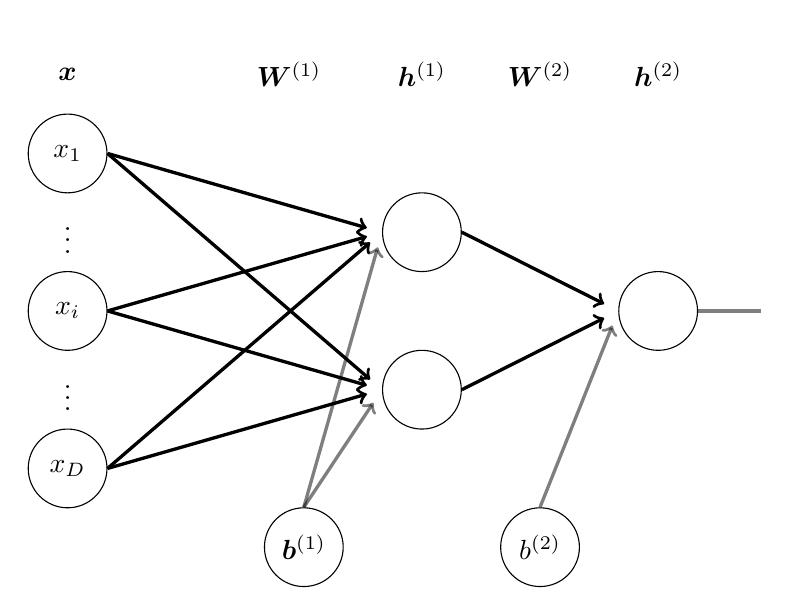
\begin{tikzpicture}
  \draw (0, 0) node[circle, minimum size=10mm, draw] (x1) {$x_{1}$};
  \draw ($(x1) - (0, 1)$) node[circle, minimum size=10mm] (xd1) {$\vdots$};
  \draw ($(xd1) - (0, 1)$) node[circle, minimum size=10mm, draw] (xi) {$x_{i}$};
  \draw ($(xi) - (0, 1)$) node[circle, minimum size=10mm] (xd2) {$\vdots$};
  \draw ($(xd2) - (0, 1)$) node[circle, minimum size=10mm, draw] (xD) {$x_{D}$};

  \draw ($(x1.north) + (0, 0.5)$) node[circle, minimum size=10mm] (x) {$\bm{x}$};
% h^(1)
  \foreach \i in{1, 2}{
    \draw ($(xd\i) + (4.5, 0)$) node[circle, minimum size=10mm, draw] (h1\i) {};
    \foreach \j in {1, i, D}{
      \draw[very thick, ->, shorten >=2mm] (x\j.east) -- (h1\i.west);
    }
  }
  \draw ($(h11.north) + (0, 1.5)$) node[circle, minimum size=10mm] (h1) {$\bm{h}^{(1)}$};

  \draw ($(h12) - (1.5, 2)$) node[circle, minimum size=10mm, draw] (b1) {$\bm{b}^{(1)}$};

  \foreach \i in {1, 2}{
    \draw[very thick, ->, shorten >=2mm, opacity=0.5] (b1.north) -- (h1\i.west);
  }

% h^(2)
  \draw ($(h12) + (3, 1)$) node[circle, minimum size=10mm, draw] (h21) {};
  \foreach \j in {1, 2}{
    \draw[very thick, ->, shorten >=2mm] (h1\j.east) -- (h21.west);
  }
  \draw ($(h21.north) + (0, 2.5)$) node[circle, minimum size=10mm] (h2) {$\bm{h}^{(2)}$};

  \draw ($(h21) - (1.5, 3)$) node[circle, minimum size=10mm, draw] (b2) {$b^{(2)}$};

  \draw[very thick, ->, shorten >=2mm, opacity=0.5] (b2.north) -- (h21.west);

  \draw ($(h1)!0.375!(x)$) node[circle, minimum size=10mm] {$\bm{W}^{(1)}$};
  \draw ($(h1)!0.5!(h2)$) node[circle, minimum size=10mm] {$\bm{W}^{(2)}$};

  \draw[very thick, shorten >=2mm, opacity=0.5] (h21.east) -- ++(1, 0);
\end{tikzpicture}
\end{figure*}
\begin{align*}
  \bm{W}^{(1)} &= \underbrace{\begin{bmatrix}
                   \text{---} &\bm{w}^{(1)}_{1}  &\text{---} \\
                   \text{---} &\bm{w}^{(1)}_{2} &\text{---}
                 \end{bmatrix}}_{2 \times D}, &\bm{b}^{(1)} &= \begin{bmatrix}
                                                  b^{(1)}_{1} \\
                                                  b^{(1)}_{2}
                                                 \end{bmatrix} \\
  \bm{W}^{(2)} &= \begin{bmatrix}
                   w^{(2)}_{1} & w^{(2)}_{2}
                 \end{bmatrix}, &\quad b^{(2)} &
\end{align*}
We have that $A \leq \sum_{i = 1}^{D} x_{i} \leq B$ iff
\begin{itemize}
\item $\sum_{i = 1}^{D} x_{i} \leq A \iff A - \sum_{i = 1}^{D} x_{i} \geq 0$ and
\item $\sum_{i = 1}^{D} x_{i} \geq B \iff \sum_{i = 1}^{D} x_{i} - B \geq 0$.
\end{itemize}
Knowing that
\begin{equation*}
  \bm{h}^{(1)} = \relu \left( \bm{W}^{(1)} \bm{x} + \bm{b}^{(1)} \right) = \begin{bmatrix}
                                                                             \relu \left( \bm{w}^{(1)}_{1} \bm{x} + b^{(1)}_{1} \right) \\
                                                                             \relu \left( \bm{w}^{(1)}_{2} \bm{x} + b^{(1)}_{2} \right)
                                                                           \end{bmatrix}
                                                                         \end{equation*}
We can set $\bm{W}^{(1)} = \begin{bsmallmatrix} -1 &\cdots &-1 \\
                       1 &\cdots &1 \end{bsmallmatrix}$ and $\bm{b}^{(1)} = \begin{bsmallmatrix}
                                                                          A \\
                                                                          -B                                                                       \end{bsmallmatrix}$ to get
\begin{equation*}
  \bm{h}^{(1)} = \begin{bmatrix}
                   \relu \left( A - \sum_{i = 1}^{D} x_{i} \right) \\
                   \relu \left( \sum_{i = 1}^{D} x_{i} - B \right)
                 \end{bmatrix}
\end{equation*}
which results in
\begin{equation*}
  \bm{h}^{(1)} = \begin{bmatrix}
                   h^{(1)}_{1} \\
                   h^{(1)}_{2}
                 \end{bmatrix} \text{where }
                 \begin{cases}
                   h_{1}^{(1)} = 0 &\text{if } \sum_{i = 1}^{D} x_{i} \geq A \\
                   h_{1}^{(1)} > 0 &\text{if } \sum_{i = 1}^{D} x_{i} < A \\
                   h_{2}^{(1)} = 0 &\text{if } \sum_{i = 1}^{D} x_{i} \leq B \\
                   h_{2}^{(1)} > 0 &\text{if } \sum_{i = 1}^{D} x_{i} > B
                 \end{cases}
\end{equation*}
In order to learn the function, we just need to choose $\bm{W}^{(2)}$ and $b^{(2)}$ such that
\begin{align*}
  \bm{h}^{(2)} &= \begin{cases}
                    +1 &\text{if } \bm{h}^{(1)} =  \begin{bsmallmatrix}
                                                     0 \\
                                                     0
                                                   \end{bsmallmatrix} \\
                    -1 &\text{otherwise}
                  \end{cases} \\
\end{align*}
equivalently
\begin{itemize}
\item $\bm{W}^{(2)} \bm{h}^{(1)} + b^{(2)} \geq 0$ when $\bm{h}^{(1)} = \begin{bsmallmatrix} 0 \\ 0 \end{bsmallmatrix}$
\item $\bm{W}^{(2)} \bm{h}^{(1)} + b^{(2)} < 0$ when $\bm{h}^{(1)} \neq \begin{bsmallmatrix} 0 \\ 0 \end{bsmallmatrix}$
\end{itemize}
Knowing that $h^{(1)}_{1} \geq 0$ and $h^{(1)}_{2} \geq 0$ we just need to set  $\bm{W}^{(2)} = \begin{bmatrix} - 1 & -1 \end{bmatrix}$ and $b^{(2)} = 0$, from which we get $\bm{W}^{(2)} \bm{h}^{(1)} + b^{(2)}$ equal to $0$ when $\bm{h}^{(1)} = \begin{bsmallmatrix} 0 \\ 0 \end{bsmallmatrix}$, and negative otherwise.

and so we learn our desired function with the weights and biases:
\begin{align*}
  \bm{W}^{(1)} &= \underbrace{\begin{bmatrix}
                   -1 &\cdots  &-1 \\
                   1 &\cdots &1
                 \end{bmatrix}}_{2 \times D}, &\bm{b}^{(1)} &= \begin{bmatrix}
                                                  A \\
                                                  -B
                                                 \end{bmatrix} \\
  \bm{W}^{(2)} &= \begin{bmatrix}
                   -1 & -1
                 \end{bmatrix}, & b^{(2)} = 0
\end{align*}
\end{document}